%!TEX root = ../08-Interference.tex
\chapter{Grating Spectroscopy}
This experiment uses interference at diffraction gratings to obtain optical spectra of elements sodium and zinc.

\section{Adjustment}
\begin{figure}
	\centering
	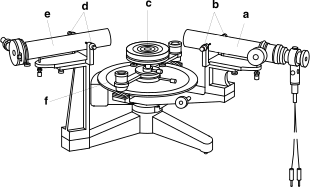
\includegraphics[width=0.6\textwidth]{./img/grating-spec.pdf}
	\caption[\texttt{LEYBOLD} grating spectrometer]{\texttt{LEYBOLD} grating spectrometer. \textbf{a}-telescope, \textbf{c}-grating fixture, \textbf{e}-collimator with adjustable slit}
	\label{fig:spec}
\end{figure}
To guarantee highest precision of subsequent measurements, the \texttt{LEYBOLD} grating spectrometer (\autoref{fig:spec}) has to be adjusted properly.

\textbf{Fixture}\\
As the horizontal inclination of the grating fixture is limited, it should be placed as horizontally as possible to leave a margin in both directions.
The same process has to be applied to the collimator and telescope while making sure the telescope's crosshair and the slit are in the focal plane of their respective objective.

\textbf{Adjusting the Telescope to Infinity}\\
To guarantee the incident light rays to enter the telescope approximately parallelly, it has to be adjusted to infinity (telescopic beam path).
This is accomplished by focusing an object at a distance of $>\SI{500}{\meter}$.

\section{Determination of the Grating Constant}\label{sec:grating}
\subsection{Theory}
Noting that gratings are just $n$ subsequent slits placed in intervals of $\frac{1}{g}$, it can be deduced that
\begin{align}
	\frac{1}{g}=\frac{\sin\phi}{n\cdot\lambda},\quad(n\in\mathbb{N}) \label{eq:grating-const}
\end{align}
holds for the maxima of the diffraction pattern.
This relation can be used to compute the grating constant of a non specified lattice.
\subsection{Setup}
The setup consists of a sodium vapor lamp whose light is pointed into the slit of the grating spectrometer.
The mean wavelength of both sodium D-lines is specified to be \SI{589.3}{\nm}.
Interference maxima of up to second order are measured, as higher orders do not exist.

\subsection{Evaluation}
\begin{table}[b!]
	\centering
	\caption[Maxima of the diffraction pattern and resulting grating constant]{Maxima of the diffraction pattern and resulting grating constant, $\lambda=\SI{589.3}{\nm}$}
	\label{tab:grating-const}
	\begin{tabular}{S|SSS|S}
		\toprule
		{order $n$}	&	{angle left $\phi_\text{L}$}	&	{angle right $\phi_\text{R}$}	&	{$\overline{\phi}$}	&	{grating constant $\frac{1}{g}$}\\
		\midrule
			1	&	\SI{201}{\degree}\SI{57}{\arcminute}	&	\SI{158}{\degree}\SI{55}{\arcminute}	&	\SI{21}{\degree}\SI{31}{\arcminute}	&	\SI{622.5}{\per\mm}	\\
			2	&	\SI{225}{\degree}\SI{20}{\arcminute}	&	\SI{133}{\degree}\SI{38}{\arcminute}	&	\SI{45}{\degree}\SI{57}{\arcminute}	&	\SI{609.8}{\per\mm}	\\
		\midrule
		{mean grating constant}	&	\SI{616.2(64)}{\per\mm}\\
		\bottomrule
	\end{tabular}
\end{table}

\autoref{tab:grating-const} shows the measured angles of features.
Using \autoref{eq:grating-const}, the mean grating constant is determined as \SI{616.2(89)}{\per\mm}, where the uncertainty is purely statistical.
As specified in the lab description, the grating's constant is supposed to be roughly \SI{600}{\per\mm}, so the measured value is satisfactory.
\todo{something something center at 180 deg, also maybe reference the tables}

\section{Wavelength Gap Between Sodium D-lines}
\begin{table}[b!]
	\centering
	\caption[Wavelength gap between sodium D-lines]{Wavelength gap between sodium D-lines, using the experimentally determined grating constant of \SI{615.7}{\per\mm}}
	\label{tab:wavelength-gap}
	\begin{tabular}{SS|SS}
		\toprule
		{angle 1 $\phi_1$}	&	{angle 2 $\phi_2$}	&	{$\Delta\phi$}	&	{$\Delta\lambda$}\\
		\midrule
			\SI{225}{\degree}\SI{19}{\arcminute}	&	\SI{225}{\degree}\SI{21}{\arcminute}	&	\SI{2}{\arcminute}	&	\SI{307}{\pm}	\\
			\SI{134}{\degree}\SI{28}{\arcminute}	&	\SI{134}{\degree}\SI{32}{\arcminute}	&	\SI{4}{\arcminute}	&	\SI{596}{\pm}	\\
		\midrule
		{mean wavelength gap}	&	\SI{452(144)}{\pm}\\
		\bottomrule
	\end{tabular}
\end{table}
To determine the wavelength gap between the $D_1$ and $D_2$ lines of sodium, the same setup as in \autoref{sec:grating} is used.
Both lines are aimed at with the crosshair and their respective angles are measured.
\autoref{tab:wavelength-gap} shows the acquired data.
Again, using \autoref{eq:grating-const}, the mean wavelength gap is calculated as $\Delta\lambda=\SI{452(144)}{\pm}$, however the statistical significance of this value is questionable, as the standard deviation almost makes up roughly 32\% of the mean value.
Nevertheless, the mean value deviates from the literature value\footnote{\url{de.wikipedia.org/wiki/Natrium-D-Linie}} of $\Delta\lambda_\text{lit}=\SI{597.4}{\pm}$ by \num{24.3}\%, which is an acceptable deviation.

\section{Determination of the Second Grating Constant}
The same deliberations as in \autoref{sec:grating} can be applied to determine the grating constant of a second lattice, only this time, higher orders are visible as the grating constant is supposed to be roughly \SI{140}{\per\mm}.
As shown in \autoref{tab:grating-const-2}, orders of up to six can be measured, as higher orders become increasingly dim.
However, six orders are enough to determine a statistically significant value of \SI{163.66(13)}{\per\mm} out of this experimental data.
This confirms the expectations for the grating constant of the second lattice.
The spectrometer's resolution would make it possible to resolve the sodium D-lines from the first maximum if the whole grating would be illuminated evenly.
However, this is not the case, so the lines can be resolved only from the fifth maximum.
\begin{table}[b!]
	\centering
	\caption[Maxima of the diffraction pattern and resulting second grating constant]{Maxima of the diffraction pattern and resulting second grating constant, $\lambda=\SI{589.3}{\nm}$}
	\label{tab:grating-const-2}
	\begin{tabular}{S|SSS|S}
		\toprule
		{order $n$}	&	{angle left $\phi_\text{L}$}	&	{angle right $\phi_\text{R}$}	&	{$\overline{\phi}$}	&	{grating constant $\frac{1}{g}$}\\
		\midrule
		1	&	\SI{185}{\degree}\SI{33}{\arcminute}	&	\SI{174}{\degree}\SI{30}{\arcminute}	&	\SI{5}{\degree}\SI{32}{\arcminute}	&	\SI{163.4}{\per\mm}	\\
		2	&	\SI{191}{\degree}\SI{8}{\arcminute}	&	\SI{168}{\degree}\SI{53}{\arcminute}	&	\SI{11}{\degree}\SI{1}{\arcminute}	&	\SI{163.7}{\per\mm}	\\
		3	&	\SI{196}{\degree}\SI{48}{\arcminute}	&	\SI{163}{\degree}\SI{9}{\arcminute}	&	\SI{16}{\degree}\SI{50}{\arcminute}	&	\SI{163.7}{\per\mm}	\\
		4	& \SI{202}{\degree}\SI{38}{\arcminute}	&	\SI{157}{\degree}\SI{15}{\arcminute}	&	\SI{22}{\degree}\SI{42}{\arcminute}	&	\SI{163.7}{\per\mm}	\\
		5	&	\SI{208}{\degree}\SI{44}{\arcminute}	&	\SI{151}{\degree}\SI{2}{\arcminute}	&	\SI{28}{\degree}\SI{51}{\arcminute}	&	\SI{163.8}{\per\mm}	\\
		6	&	\SI{215}{\degree}\SI{12}{\arcminute}	&	\SI{144}{\degree}\SI{27}{\arcminute}	&	\SI{35}{\degree}\SI{23}{\arcminute}	&	\SI{163.7}{\per\mm}	\\
		\midrule
		{mean grating constant}	&	\SI{163.66(13)}{\per\mm}\\
		\bottomrule
	\end{tabular}
\end{table}
